\documentclass[a4paper,14pt]{extarticle}
\usepackage{fontspec, unicode-math}
\usepackage[english, russian]{babel}
\setmainfont{Times New Roman}
\setmonofont{CMU Typewriter Text}

\usepackage{enumitem}
\usepackage{alltt}

\usepackage{graphicx}
\usepackage{float}
\usepackage{caption}
\captionsetup[figure]{name={Рисунок}}

\usepackage{nameref}

\usepackage{makecell}
\renewcommand\theadfont{\bfseries}
\renewcommand\theadalign{cl}

% === WIP ===

\usepackage{xcolor}
\newcommand{\todo}[1]{\textbf{\textcolor{red}{#1}}}

% === Page Setup ===

\usepackage[top=20mm, bottom=20mm, left=25mm, right=10mm]{geometry}
\usepackage[nodisplayskipstretch]{setspace}
\onehalfspacing %\setstretch{1.5}

\usepackage{indentfirst}
\setlength{\parindent}{1.25cm}

% Avoid overfull boxes by stretching word spacing
\setlength\emergencystretch{\hsize}

% === Formatting ===

\usepackage{titlesec}
\titleformat{\section}[block]{\centering\bfseries\large}{\arabic{section}}{1ex}{\MakeUppercase}
\titleformat{\subsection}[block]{\hspace{\parindent}\bfseries\normalsize}{\arabic{section}.\arabic{subsection}}{1ex}{}
\titleformat{\subsubsection}[block]{\hspace{\parindent}\bfseries\normalsize}{\arabic{section}.\arabic{subsection}.\arabic{subsubsection}}{1ex}{}
\titlespacing*{\section}{0pt}{36pt}{36pt}

% === Table of Contents ===

\addto\captionsrussian{
  \renewcommand{\contentsname}{Оглавление}
}

% Show dots for all entries
\usepackage[titles]{tocloft}
\renewcommand{\cftsecleader}{\cftdotfill{\cftdotsep}}
% Remove bold style for section names/page numbers
\renewcommand{\cftsecfont}{\normalfont}
\renewcommand{\cftsecpagefont}{\normalfont}
% Reduce spacing between entries
\setlength{\cftbeforesecskip}{10pt}

% === Bibliography ===

\usepackage[parentracker=true,
  backend=biber,
  language=russian,
  autolang=other,
  sorting=none,
  citestyle=gost-numeric,
  bibstyle=gost-numeric,
]{biblatex}
\addbibresource{thesis.bib}

\usepackage{xurl}
\usepackage[hidelinks]{hyperref}

% === Lists ===

\makeatletter
\AddEnumerateCounter{\asbuk}{\russian@alph}{щ}
\makeatother
\newlist{ol}{enumerate}{2}
\setlist[ol,1]{noitemsep,topsep=0em,label=\arabic*),ref=\arabic*}
\setlist[ol,2]{noitemsep,topsep=0em,label=\asbuk*),ref=\asbuk*}

\newlist{ul}{itemize}{1}
\setlist[ul,1]{noitemsep,topsep=0em,label=\textendash,ref=\textendash}

% === Custom Commands ===

\newcommand{\topic}[1]{\textbf{#1.}}

\newcommand{\var}[1]{\mathop{\mathit{#1}}}

% === Body ===

\begin{document}

\tableofcontents

\newpage
\section*{ТЕРМИНЫ И ОПРЕДЕЛЕНИЯ}
\phantomsection\addcontentsline{toc}{section}{ТЕРМИНЫ И ОПРЕДЕЛЕНИЯ}

Шейдер — программа, предназначенная для исполнения на графическом процессоре

\newpage
\section*{ВВЕДЕНИЕ}
\phantomsection\addcontentsline{toc}{section}{ВВЕДЕНИЕ}

\topic{Актуальность темы исследования} Графические процессоры получили широкое применение
в задачах машинного обучения. Для достижения оптимальной утилизации аппаратных ресурсов
алгоритмы реализуются при помощи ассемблера. Отсутствие средств верификации ассемблерных
программ для ГП затрудняет разработку и может привести к некорректным результатам во время исполнения.

Особый интерес представляют графические процессоры AMD, которые предоставляют разработчику
на ассемблере доступ к аппаратному набору команд. В связи с особенностями аппаратной
реализации от программиста требуется ручное разрешение зависимостей по данным.

Ошибки в разрешении зависимостей могут быть обнаружены методами статического анализа
еще на этапе разработки программы. Задача осложняется тем, что при разработке
на ассемблере используются различные препроцессоры и трансляторы кода. В работе
предлагается анализ исполняемых файлов, который позволяет работать с единым
представлением программы, которое не зависит от инструментов, используемых при разработки.\\

\topic{Степень теоретической разработанности темы} Статический анализ исполняемых файлов
широко рассмотрен в работах, посвященных информационной безопасности, а именно:
дизассемблированию обфусцированного кода и обнаружению вирусов,
проверке недоверенного кода в плагинах на некорректный доступ к памяти и т.д.\cite{static-analysis-binary}

Существующие средства статического анализа для графических процессоров работают с
высокоуровневыми языками (CUDA, OpenCL) и направлены на обнаружение ошибок,
не отслеживаемых компиляторами — например, состояний гонки, в которых несколько потоков
записывают и читают одни и те же данные в памяти без синхронизации\cite{gpu-static-verification}.

Вопросу применения статического анализа исполняемых файлов к шейдерам существенного внимания
не уделяется, поскольку разработка ассемблерных программ, оптимизированных для конкретных ГП,
менее распространена и зачастую выполняется проприетарно.\\

\textbf{Целью работы} является снижение трудозатрат на разработку ассемблерных шейдеров
путем создания средства статического анализа исполняемых файлов для графических процессоров.\\

\textbf{Задачи:}
\begin{ul}
\item Изучение архитектурных особенностей графических процессоров AMD с целью выделения
круга задач, решаемых статическим анализом.
\item Исследование открытых средств статического анализа исходного кода, в особенности
компиляторов, для ознакомления с современными подходами (алгоритмами).
\item Разработка программного средства статического анализа исполняемых файлов
на основании проведенного исследования.
\item Тестирование работоспособности системы на существующих ассемблерных шейдерах
с намеренно внесенными ошибками.
\end{ul}\ %

\textbf{Объектом исследования} в работе выступают методы статического анализа кода
в применении к исполняемым файлам для графических процессоров.\\

\textbf{Практическая значимость:} разработанная в ходе работы система
статического анализа применима в процессах разработки ассемблерных шейдеров
для обнаружения ряда ошибок на ранних этапах разработки. Результаты работы
могут служить основой дальнейших исследований в области статического анализа
и верификации программ для графических процессоров.

\newpage
\section{Обзор предметной области}

\subsection{Неспециализированные вычисления на графических процессорах}

Графические процессоры широко применяются для неспециализированных вычислений —
\textit{general-purpose computing on graphics processing units, GPGPU}.
Особый интерес представляют математические расчеты, используемые в
\textit{сверточных нейронных сетях} — методе машинного обучения, в основе которого
лежат матричные операции свертки, субдискретизации (\textit{pooling}) и т.п.
Производительность графических ускорителей в выполнении подобных операций
значительно превышает производительность центральных процессоров.\\

Для исполнения неспециализированных вычислений требуются специальные платформы,
которые выполняют несколько задач:
\begin{ul}
\item Преобразование исходных текстов на определенном языке программирования
  в исполняемый файл, содержащий инструкции для графического процессора и метаданные о программе.
\item Предоставление библиотек математических примитивов (BLAS, FFT)
  для использования в вычислительных шейдерах.
\item Предоставление набора интерфейсов для запуска программ на ГП, перемещения данных между
  оперативной памятью и выделенной памятью ускорителя, выполнения других операций.
\item Обеспечение взаимодействия между драйвером ускорителя и пользовательской программой,
  использующей интерфейсы платформы.
\end{ul}\ %

Компания NVIDIA предоставляет для своих ускорителей платформу \textit{CUDA}. Прямым аналогом
со стороны AMD является \textit{ROCm}. Вычислительные шейдеры могут составляться как
на высокоуровневых языках (C++11, OpenCL), так и на ассемблере. Платформа доступна
только на операционной системе Linux.

\subsection{Исполнение шейдеров на графических процессорах}

Графические процессоры достигают высокой производительности в математических операциях
за счет реализации модели выполнения \textit{SIMT} (одиночный поток команд, множество потоков).
Программа разделяется на множество потоков исполнения (\textit{workitems}),
каждый из которых может следовать произвольному пути в программе.

В графических процессорах AMD\footnote{Здесь и далее при обсуждении графических процессоров AMD
подразумеваются архитектуры GCN и CDNA, которые используются в ускорителях для высокопроизводительных
вычислений и машинного обучения. Современные ГП общего назначения строятся на базе архитектуры RDNA,
которая обладает рядом отличий: возможностью исполнения 32 потоков, разделенным счетчиком векторных
операций с памятью и т.д.}
одна и та же инструкция в программе исполняется одновременно на наборе из 64 потоков,
именуемом \textit{wavefront}. Инструкции делятся на два вида: векторные и скалярные.
Векторные операции применяются к значениям в каждом потоке за счет использования SIMD АЛУ.
Скалярные операции применяются к одному значению на весь набор потоков.

Рабочие данные хранятся в скалярных, \textit{SGPR}, и векторных, \textit{VGPR},
32-разрядных регистрах общего назначения. Программа может использовать до 102
SGPR (\verb|s0| — \verb|s101|) и до 256 VGPR ({\verb|v0| — \verb|v255|).

\subsubsection{Управление потоком выполнения программы}
\label{section:gcn-program-flow}

Ветвление в шейдерах осуществляется двумя способами: изменением счетчика команд скалярными
инструкциями и маскированием потоков векторными инструкциями сравнения\cite{vega-isa}.
Маскирование заключается в изменении маски активности (\textit{EXEC}), каждый бит которой
соотвествует отдельному потоку. Для потоков с нулевым битом векторные операции интерпретируются как NOP.
Если все биты в маске активности равны нулю, векторные инструкции не пропускаются.

Скалярные инструкции управления потоком выполнения разделяются на несколько видов:
\begin{ol}
\item Команды прямого перехода, в которых кодируется целевой адрес как смещение относительно счетчика команд:
  \begin{ul}
  \item безусловный переход (\verb|s_branch|);
  \item условный переход (\verb|s_cbranch_*|);
  \item вызов функции (\verb|s_call_b64|): перед переходом значение счетчика команд
  сохраняется в паре регистров общего назначения.
  \end{ul}
\item Команды косвенного перехода, которые считывают целевой адрес из пары регистров общего назначения:
  \begin{ul}
  \item безусловный переход (\verb|s_setpc_b64|);
  \item вызов функции (\verb|s_swappc_b64|).
  \end{ul}
\item Команды прямого (\verb|s_cbranch_i_fork|) и косвенного (\verb|s_cbranch_g_fork|)
  условного перехода по маске. Переход по адресу осуществляется только для потоков, которые соответствует
  маски-операнду; адрес следующей инструкции и инверсия маски-операнда сохраняются в стек
  (в качестве стека используются регистры общего назначения, по 4 регистра на один переход).
  Команда \verb|s_cbranch_join| размещается в конце блока, в пределах которого осуществляется ветвление.
  Она снимает со стека адрес следующего перехода и соответсвующую маску активности и применяет их.
\item Команда переключения режима пропуска векторных инструкций \verb|s_setvskip|. В режиме
  \textit{VSKIP} все векторные инструкциии пропускаются; векторные операции с памятью не выполняются
  и не инкрементируют счетчики незавершенных операций.
\item Команда завершения выполнения программы \verb|s_endpgm|. Перед завершением автоматически
  ожидаются все операции доступа к памяти.
\end{ol}

\subsubsection{Ожидание готовности данных при запросах к памяти}
\label{section:gcn-waitcnt}

Как и в центральных процессорах, время доступа к памяти в графических ускорителях
значительно превышает время выполнения арифметико-логических инструкций.
Для сокращения простоя в современных ЦП используется внеочередное исполнение, при котором
инструкции выполняются не в порядке следования в программе, а в порядке доступности операндов.
В ГП для скрытия задержки используется иной механизм: при ожидании данных одним набором
потоков исполнение переходит к следующему\cite{gcn-performance}.

Тем не менее, количество наборов потоков, между которыми передается управление, ограничено
аппаратными ресурсами — в частности, объемом регистрового файла для хранения состояния каждого
исполняемого набора. В связи с этим операции с памятью в архитектуре ГП AMD асинхронны.
После запроса на чтение или запись программист может вставить несвязанные инструкции,
сократив время простоя АЛУ. Требование готовности данных обозначается специальной
инструкцией \verb|s_waitcnt|, <<ожидание значения счетчика>>.

Предусмотрено три счетчика операций:
\begin{ul}
\item \verb|vmcnt| для векторных операций с глобальной памятью;
\item \verb|lgkmcnt| для скалярных операций с глобальной памятью и векторных операций с локальной памятью;
\item \verb|expcnt| для векторных операций записи в общую память.
\end{ul}

После каждой операции с памятью соответствующий счетчик инкрементируется, а по завершении
операции — декрементируется. Операции одного типа завершаются в порядке очереди, что
позволяет ожидать готовности только тех данных, которые необходимы для вычислений в данный
момент. Если же счетчик содержит операции различных типов, или какая-либо из операций
характеризуется внеочередным завершением (скалярный доступ к памяти), то очередность не гарантируется.
В таком случае программист должен ожидать обуления соответствующего счетчика.

Инструкция ожидания \verb|s_waitcnt| кодирует значение счетчика, до достижения
которого исполнение программмы приостанавливается. В инструкции выделено 6 бит под значение
\verb|vmcnt|, 3 бита под значение \verb|expcnt|, 4 бита под значение \verb|lgkmcnt|.
Если все биты счетчика выставлены в 1, то его значение не ожидается. Таким образом,
выражение ожидания может содержать разные значения для одного или нескольких счетчиков,
например: \verb|s_waitcnt vmcnt(1) lgkmcnt(2)|. Команду
\verb|s_waitcnt vmcnt(0) lgkmcnt(0) expcnt(0)|, которая соответствует ожиданию всех
незавершенных операций, принято сокращать как \verb|s_waitcnt 0|.

\subsubsection{Разрешение конфликтов по данным}
\label{section:gcn-wait-states}

Существует также ряд зависимостей по данным, не связанных с доступом к памяти,
которые не отслеживаются графическим процессором из-за особенностей аппаратной реализации.
В официальном руководстве к архитектуре GCN таких ситуаций определено 16\cite[Глава~4.5]{vega-isa}.
Архитектура CDNA, на которой основывается передовой ускоритель вычислений \textit{AMD Instinct MI100},
добавляет к этому 21 ситуацию, относящуюся к матричным операциям\cite[Глава~7.2]{cdna-isa}.

При наличии конфликта по данным программист или компилятор должны обеспечить определенное
количество независимых операций между зависимыми инструкциями. Если независимые операции
в данном участке программы отсутствуют, вставляется инструкция \verb|s_nop <waits>|,
где \verb|<waits> + 1| — число слотов задержки, т.е. циклов, на протяжении которых
исполнение приостанавливается.

Для каждого случая ручного разрешения конфликта по данным в руководстве описываются:
\begin{ul}
\item Правило, по которому определяются зависимые инструкции. Зачастую проверяется
совпадение операндов между операциями — например, векторная инструкция,
записывающая скалярный регистр, и \verb|v_readlane|, использующая этот же
регистр в качестве селектора, зависят друг от друга.
\item Количество слотов задержки, которые необходимо обеспечить между зависимыми инструкциями.
\end{ul}

\subsection{Разрешение зависимостей при компиляции шейдеров}

При использовании высокоуровневых языков программисту не требуется следить
за ожиданием обращений к памяти и предотвращать конфликты по данным;
эту задачу берет на себя компилятор. Перед изучением используемых алгоритмов
разрешения зависимостей необходимо ознакомиться с общими принципами работы
современных компиляторов.

Поддержка различных языков программирования и целевых платформ осуществляется
за счет выделения независимых фаз компиляции, которые реализуются отдельными модулями.
Выделяют три основных модуля\cite[Глава~1]{compilers}:

\begin{ul}
\item \textit{фронтэнд} (\textit{frontend}), отвечающий за трансляцию исходного текста программы в
  промежуточное представление;
\item \textit{оптимизатор} (\textit{optimizer}), выполняющий различные преобразования над промежуточным
  представлением, которые направлены на сокращение времени исполнения,
  уменьшение размера программы и т.д.;
\item \textit{бэкэнд} (\textit{backend}), преобразующий промежуточное представление в машинный код.
\end{ul}

Помимо промежуточного представления программы, которое передается между фазами,
модуль может использовать внутренние представления, необходимые для выполнения его функций.
Например, при чтении исходного кода программы фронтэнд создает синтаксические деревья,
а при генерации машинного кода бэкэнд работает с различными графами, моделирующими поведение
программы.

Интересующая нас задача вставки инструкций \verb|s_waitcnt| и \verb|s_nop| относится
к этапу диспетчеризации инструкций, которая производится бэкэндом над представлением программы
в виде \textit{управляющего графа} (\textit{control flow graph}).

Управляющий граф\cite{cfg-allen}\cite{cfg-ru} представляет собой ориентированный граф, вершинами которого
выступают \textit{базовые блоки} (\textit{basic blocks}) — последовательности инструкций,
не содержащие переходов в другие места программы, за исключением последней
инструкции в блоке, \textit{точки выхода}. Ребра отражают переходы в программе.
В задачах анализа важны следующие взаимосвязи вершин:
\begin{ul}
\item \textit{преемник вершины $p$} (\textit{successor of $p$}) — такая вершина $q$,
  для которой в орграфе существует путь из $p$ в $q$;
\item \textit{предшественник вершины $p$} (\textit{predecessor of $p$}) — такая вершина $q$,
  для которой в орграфе существует путь из $q$ в $p$.
\end{ul}
Стоит отметить, что одна и та же вершина $q$ может быть как преемником, так и предшественником вершины $p$,
что отражает циклическую конструкцию в программе.

Основным методом решения задач статического анализа являются итеративный подход\cite[Глава~8]{compilers}.
Каждой вершине присваивается изначальное состояние. В процессе обхода графа к каждой вершине
применяется функция, преобразующая ее текущее состояние в новое. Полученное состояние
соединяется с состоянием последующих вершин в направлении обхода, образуя их новые состояния.
Обход продолжается до тех пор, пока не будет достигнута неподвижная точка (\textit{fixed point}), т.е.
пока состояния вершин не перестанут изменяться. Конечность алгоритма анализа может гарантироваться
при условии, что домен состояний является конечным множеством, а изменение состояний происходит монотонно.

Порядок обхода графа выбирается в зависимости от решаемой задачи:
\begin{ul}
\item Анализ прямого потока данных (\textit{forward dataflow}), к которому относится отслеживание обращений
  к памяти, производится при помощи прямого обхода в глубину (\textit{preorder}; посещается блок, затем его преемники) или RPO-обхода (\textit{reverse postorder}; блок посещается после всех предшественников, за исключением тех, которые связаны с блоком обратными ребрами).

\item Анализ обратного потока данных (\textit{backward dataflow}), к которому относится проверка вставки
слотов задержки перед использованием зависимых данных, производится при помощи обратного обхода
(\textit{postorder}; посещается блок, затем его предшественники).
\end{ul}

Платформа ROCm включает в себя единый компилятор шейдеров для всех поддерживаемых
высокоуровневых языков программирования (С++, OpenCL) — \textit{Clang},
разрабатываемый как часть проекта LLVM, обладающий модульным строением, описанный выше.
За генерацию машинного кода для графических процессоров AMD в \textit{Clang} отвечает бэкэнд AMDGPU.
Рассмотрим подробнее его работу в LLVM версии 12\cite{llvm-12}.

\subsubsection{Обработка запросов к памяти в компиляторе LLVM}
\label{section:gcn-waitcnt-llvm}

Вставка инструкций \verb|s_waitcnt| производится классом \verb|SIInsertWaitcnts|,
который наследуется от \verb|MachineFunctionPass|, т.е. является преобразованием
(проходом), выполняемым во время генерации кода над инструкциями каждой функции программы.

\verb|SIInsertWaitcnts| реализует итеративный алгоритм анализа прямого потока данных.
Обход управляющего графа осуществляется в RPO-порядке. Каждому из блоков присваивается
объект \verb|WaitcntBrackets|, отслеживающий:
\begin{ul}
\item число всех обращений к памяти для каждого из счетчиков операций
  (\verb|vmcnt|, \verb|lgkmcnt|, \verb|expcnt|) — $\var{ScoreUb}$;
\item число завершенных операций для каждого из счетчиков (согласно
  вставленным инструкциям \verb|s_waitcnt|) — $\var{ScoreLb}$;
\item номер последней операции, использующей регистр, для всех регистров
  в программе (отсутствию операций соответствует значение $0$) — $\var{VgprScores}$, $\var{SgprScores}$.
\end{ul}

Функция обновления состояния блока посещает каждую инструкцию в блоке в порядке
исполнения. При этом выполняется следующая последовательность действий:
\begin{ol}
\item Проверяются случаи, в которых необходимо вставить ожидание:
  \begin{ol}
  \item при выходе из функции (\verb|s_setpc_b64|) ожидаются все операции;
  \item если операнд инструкции является скалярным регистром $s$, который используется в
    незавершенной операции, т.е. выполняется $\var{SgprScores}[s] > \var{ScoreLb}[\mathtt{lgkmcnt}]$:
    \begin{ul}
    \item при наличии незавершенных операций \verb|flat| согласно архитектуре набора
      команд\cite[Глава~9.2.2]{vega-isa} вставляется \verb|s_waitcnt 0|;
    \item иначе вставляется \verb|s_waitcnt lgkmcnt(0)|, поскольку скалярные операции с памятью
      выполняются вне очереди;
    \end{ul}
  \item если операнд инструкции является векторным регистром $v$, участвующим
    в незавершенной операции, т.е. выполняются условия 
    $\var{VgprScores}[\mathtt{vmcnt}][v]>\var{ScoreLb}[\mathtt{vmcnt}]$ или
    $\var{VgprScores}[\mathtt{lgkmcnt}][v]>\var{ScoreLb}[\mathtt{lgkmcnt}]$:
    \begin{ul}
    \item при наличии незавершенных операций \verb|flat| согласно архитектуре набора
      команд вставляется \verb|s_waitcnt 0|;
    \item если операция входит в счетчик \verb|vmcnt|, то вставляется \verb|s_waitcnt vmcnt(w)|,
      где $w = \var{ScoreUb}[\mathtt{vmcnt}] - \var{VgprScores}[\mathtt{vmcnt}][v]$;
    \item если операция входит в счетчик \verb|lgkmcnt| и имеет тот же тип, что и все
      незавершенные операции в счетчике, то вставляется \verb|s_waitcnt vmcnt(w)|,
      где $w = \var{ScoreUb}[\mathtt{lgkmcnt}] - \var{VgprScores}[\mathtt{lgkmcnt}][v]$;
    \item иначе вставляется \verb|s_waitcnt lgkmcnt(0)|, поскольку скалярные операции с памятью
      выполняются вне очереди.
    \end{ul}
  \end{ol}
\item Если необходимо добавить ожидания:
  \begin{ul}
  \item при наличии в блоке предшествующей инструкции \verb|s_waitcnt| ожидание объединяется
    с предшествующей инструкцией, иначе в блок вставляется новая инструкция \verb|s_waitcnt|;
  \item обновляется число завершенных операций ($\var{ScoreLb}$) для счетчиков,
    которые входят в выражение ожидания.
  \end{ul}
\item Если рассматриваемая инструкция является обращением к памяти,
  число обращений к памяти ($\var{ScoreUb}$) инкрементируется, и полученное значение
  присваивается номеру операции регистра назначения ($\var{VgprScores}$ или $\var{SgprScores}$).
\end{ol}

Функция соединения, которая обновляет состояния всех преемников рассматриваемого блока,
подсчитывает незавершенные операции в исходном и новом состоянии, и обновляет
счетчики согласно наибольшим значениям, т.е. изменение состояний происходит монотонно.

Исследование принципа работы используемого алгоритма позволяет заключить, что он обладает
следующими ограничениями:
\begin{ul}
\item в некоторых случаях (например, перед возвратом из функции) вставляются слишком
  строгие ожидания, что может привести к ненужному простою АЛУ;
\item отслеживается только числовое значение счетчиков — алгоритм не позволяет
  определить, для каких обращений к памяти необходима вставка конкретной
  инструкции \verb|s_waitcnt|.
\end{ul}

\subsubsection{Вставка слотов задержки в компиляторе LLVM}
\label{section:gcn-wait-states-llvm}

Разрешение зависимостей со вставкой слотов задержки выполняется в LLVM на этапе
диспетчеризации инструкций. За это отвечают классы, наследуемые от \verb|ScheduleHazardRecognizer|.
Для каждой инструкции вызывается метод \verb|getHazardType|, который проверяет наличие
конфликтов. Метод может вернуть три значения:
\begin{ol}
\item \verb|NoHazard| означает, что инструкция может быть помещена в данном участке программы;
\item \verb|Hazard| указывает на то, что текущее размещение инструкции приведет к аппаратной
  задержке исполнения (\textit{stall}) — при наличии других инструкций, которые
  могут быть помещены в данный участок, диспетчер выберет их;
\item \verb|NoopHazard| указывает на то, что инструкция не может быть размещена в данном
  участке — диспетчер должен выбрать другие доступные инструкции или вставить слоты задержки.
\end{ol}
При нахождении \verb|NoopHazard| затем вызывается метод \verb|PreEmitNoops|, который возвращает
количество необходимых слотов.

За обнаружение конфликтов при генерации кода для ГП AMD отвечает класс \verb|GCNHazardRecognizer|.
Метод \verb|getHazardType| вычисляет число слотов задержки, которые необходимо добавить
перед инструкцией, и возвращает \verb|NoopHazard|, если значение больше 0, иначе \verb|NoHazard|.
Метод \verb|PreEmitNoops| повторяет вычисления и возращает число необходимых слотов задержки.

Как описано в разделе \ref{section:gcn-wait-states}, класс конфликтов определяется
правилом нахождения зависимых инструкций (в коде — $\var{IsHazardFn}$) и числом
независимых операций, необходимых между ними (в коде — $\var{WaitStatesNeeded}$).

Проверка конфликтов с вычислением требуемых слотов задержки перед инструкцией $\var{I}$,
входящей в базовый блок $\var{BB}$, выполняется следующим образом:
\begin{ol}
\item Для каждой инструкции в $\var{BB}$, в обратном порядке начиная с предшествующей $\var{I}$,
определяется соответствие правилу зависимости $\var{IsHazardFn}$:
  \begin{ul}
  \item Если операция не является зависимой, вычисляется количество занимаемых ею слотов задержки
    (1 для всех инструкций кроме \verb|s_nop|, для \verb|s_nop n| составляет \verb|n| + 1)
    и прибавляется к счетчику независимых операций $\var{WaitStates}$.
  \item Если операция является зависимой, то возвращается число пропущенных слотов задержки
    как $\var{WaitStatesNeeded} - \var{WaitStates}$.
  \end{ul}
\item Если инструкция не имеет конфликтов, то есть выполняется функция $\var{IsExpired}$, в простейшем
  случае опеределенная как $\var{WaitStates} \geqslant \var{WaitStatesNeeded}$, то алгоритм завершает работу.
\item В противном случае, работа алгоритма продолжается:
  \begin{ul}
  \item Если достигнуто начало $BB$, то обхода продолжается для каждого из его предшественников,
    начиная с последней инструкции в блоке.
  \item Иначе продолжается рассмотрение следующей инструкции в обратном порядке.
  \end{ul}
\end{ol}

При исследовании реализации алгоритма было обнаружено, что для ассемблерных вставок в исходном коде шейдера
осуществляется проверка только одного класса конфликтов, описанных в руководстве к архитектуре.
Метод \verb|checkInlineAsmHazards| содержит следующий комментарий:
\begin{verbatim}
Note that this function doesn't attempt to address all
possible inline asm hazards (good luck), but is a
collection of what has been problematic thus far.
\end{verbatim}

\subsection{Ручное составление ассемблерных шейдеров}

Одной из основных целей при использовании ассемблера является сокращение времени
простоя вычислительных блоков ускорителя за счет применения ручных оптимизаций,
которые не реализуемы на высокоуровневом языке.

Наглядным примером оптимизаций является обработка запросов к памяти. Если
компилятор высокоуровневого языка лишь вставляет необходимые инструкции ожидания,
то программист на ассемблере старается также обеспечить, чтобы между запросом к памяти
и ожиданием было как можно больше несвязанных арифметических операций,
а ожидаемое значение счетчика было как можно более точным, поскольку
это увеличивает долю полезной работы. При этом повышается вероятность совершения
ошибки — пропуска необходимой инструкции из-за сложной структуры программы.

Поиск ошибок в ассемблерных шейдерах можно автоматизировать, тем самым сократив
трудозатраты на разработку. К используемым алгоритмам при этом применяются иные требования,
нежели в компиляторах. Алгоритмы должны предоставлять подробную информацию о месте
и причине возникновения ошибок; в противном случае, программист потратит значительный
объем времени на их локализацию, что сведет к минимуму преимущества автоматизации.

Средства статического анализа, используемые в средствах поддержки разработки,
опираются на исходный код или промежуточное представление (байткод) программ
\cite{static-code-analysis}. Особенности разработки ассемблерных шейдеров
для графических процессоров AMD затрудняют использование подобного подхода.

Во-первых, встречается несколько способов записи инструкций — так, руководство к бэкэнду
AMDGPU описывает два синтаксиса операндов, стандартный и альтернативный (SP3)\cite{gcn-asm-syntax}.
Помимо этого, существуют сторонние ассемблеры, отличающиеся не только синтаксисом,
но и вспомогательными возможностями, например, \textit{CLRadeonExtender}\cite{clrx}.

Во-вторых, высокоуровневые конструкции в ассемблерном коде (переменные, циклы, функции)
реализуются в виде макросов, т.е. текстовых подстановок, которые не несут в себе полезной
информации, такой как область видимости, а лишь затрудняют анализ потока управления программы.

В связи с этим, в качестве входных данных при статическом анализе ассемблерных шейдеров
следует рассматривать не исходный код, а исполняемые файлы, формат которых
на платформе ROCm строго определен бинарным интерфейсом приложений\cite{amdgpu-abi} и не
зависит от средств разработки. 

\newpage
\section{Разработка подхода к статическому анализу шейдеров}
\label{section:algorithms}

\subsection{Постановка задач, решаемых статическим анализом}

В ходе исследования предметной области были выделены две области, в которых ошибку программиста
на ассемблере может быть сложно диагностировать во время исполнения, но можно
предотвратить, внедря статическую верификацию программ:
\begin{ol}
\item \textbf{Вставка инструкций ожидания (\texttt{s\_waitcnt})}. При обращении к регистрам,
которые используются в незавершенном обращении к памяти, необходимо сформировать соответствующее
предупреждение, предоставив информацию об инструкции, читающей регистр, инструкции,
использующей регистр, и состоянии очереди запросов.
\item \textbf{Вставка слотов задержки (\texttt{s\_nop})}. При наличии конфликтов по данным
между зависимыми операциями необходимо сформировать предупреждение, которое указывает на
на зависимые инструкции, а также содержит количество недостающих слотов задержки.
\end{ol}

Разрабатываемый подход к анализу программы должен удовлетворять следующим требованиям:

\begin{ul}
\item Входными данными выступают исполняемые файлы.
\item Хотя исполняемые файлы могут содержать отладочные символы (имена меток и макросов),
в анализе они использоваться не должны, поскольку их наличие не гарантируется. Символы могут быть
намеренно удалены для уменьшения размера исполняемого файла; некоторые трансляторы ассемблерного
кода изначально не поддерживают таблицы символов.
\item Анализ производится над уравляющим графом, который восстанавливается по инструкциям перехода.
\end{ul}

\subsection{Составление алгоритмов анализа}

\subsubsection{Извлечение инструкций из исполняемого файла}

\topic{Чтение исполняемых файлов} Запуск скомпилированных шейдеров на платформе ROCm
нароизводится в среде исполнения HSA. Шейдеры загружаются из исполняемых файлов
в формате ELF, именуемых \textit{HSA Code Object (CO)}. Встречается несколько версий CO
\cite{llvm-12-amdgpu}:

\begin{ul}
\item  \textit{Code Object V2}: для каждого шейдера в таблице
глобальных символов ELF создается запись c именем шейдера и
указанием на фрагмент секции \verb|.text| c исполняемым кодом шейдера.
Первые 256 байт c начала фрагмента отводятся под структуру с метаданными,
которые включают в себя смещение исполняемых инструкций относительно начала фрагмента.
По умолчанию смещение составляет 256 байт, т.е. инструкции следуют сразу после структуры с метаданными.
\item \textit{Code Object V3} и \textit{Code Object V4}: метаданные помещаются в отдельный
фрагмент секции \verb|.rodata|, на который указывает глобальный символ \verb|<kernel name>.kd|
(\verb|<kernel name>| — имя шейдера). На каждый шейдер создается два
глобальных символа; инструкции идут с начала фрагмента в секции \verb|.text|.
\end{ul}

Таким образом, для извлечения машинного кода шейдеров применяется следующая последовательность действий:
\begin{ol}
\item Считать из исполняемого файла таблицу глобальных символов, которая содержится в секции \verb|.dynsym|.
\item Для каждого из символов $\var{KernelSym}$, данные которых содержаться в секции \verb|.text|:
  \begin{ol}
  \item Проверить, существует ли символ $\var{DescriptorSym}$, указывающий на дескриптор: его название должно состоять
    из имени шейдера и суффикса \verb|.kd|, а данные должны содержаться в секции \verb|.rodata|.
  \item Если $\var{DescriptorSym}$ существует, то используется \textit{Code Object V3/V4}. Машинный код исполняемых
    инструкций извлекается из секции \verb|.text| по смещению, записанному в $\var{KernelSym}$.
  \item Если $\var{DescriptorSym}$ не существует, то используется \textit{Code Object V2}. В таком случае необходимо:
    \begin{ul}
    \item Считать структуру метаданных \verb|amd_kernel_code_t|\cite{amdgpu-abi}
      из секции \verb|.text| по смещению, записанному в $\var{KernelSym}$.
    \item Считать значение \verb|kernel_code_entry_byte_offset|, располагающееся в байтах 16-23 структуры,
      и прибавить его ко смещению, записанному в $\var{KernelSym}$.
    \item Начиная с полученного смещения, извлечь из секции \verb|.text| машинный код исполняемых инструкций.
    \end{ul}
  \end{ol}
\end{ol}

Для упрощения подхода к анализу в последующих этапах принимается допущение,
что исполняемый файл содержит один и только один шейдер. В случае, когда в файле содержится несколько
$\var{KernelSym}$, для анализа выбирается первый из них.\\

\topic{Дизассемблирование} Задача преобразования машинного кода инструкций в их текстовое представление
осложняется особенностями архитектуры графических процессоров AMD:
\begin{ul}
\item размер инструкций может составлять 4 байта (форматы SOP2, SOP1, SOPK, SOPP, SOPC, SMRD, VOP2, VOP1, VOPC, VINTRP)
  или 8 байт (форматы SMEM, VOP3A, VOP3B, VOP3P, DS, MUBUF, MTBUF, MIMG);
\item некоторые форматы инструкций (VOP1, VOP2, VOPC) поддерживают 32-разрядные константные операнды,
  записываемые после инструкции;
\item кодирование инструкций может различаться между семействами графических процессоров.
\end{ul}

Проект LLVM предоставляет дизассемблер для набора команд графических процессоров AMD,
использование которого позволяет преодолеть обозначенные трудности. Взаимодействие с
дизассемблером AMDGPU обсуждается в разделе~\ref{section:impl-disasm}.

\subsubsection{Восстановление потока управления}

\topic{Выделение базовых блоков} Первым шагом при построении управляющего графа
является определение вершин — базовых блоков. Для выполнения этой задачи
строится множество адресов начала блоков, $\var{Leaders}$. Изначально
оно содержит адрес начала программы. Затем инструкции в программе
последовательно проверяются на соответствие скалярным командам ветвления
(см. раздел~\ref{section:gcn-program-flow}).

Для каждой найденной команды перехода в $\var{Leaders}$ помещается адрес следующей инструкции,
$NextPc$. Таким образом гарантируется, что инструкции перехода всегда завершают базовый
блок. Впоследствии могут быть обнаружены и отброшены недостижимые блоки, к примеру,
содержащие инструкции, которые следуют за завершением программы (\verb|s_endpgm|).

$NextPc$ равен значению счетчика команд на момент исполнения инструкции перехода.
Его можно вычислить, прибавив размер инструкции перехода к ее адресу; размер инструкций
\verb|s_branch|, \verb|s_cbranch_*|, \verb|s_call_b64|, \verb|s_setpc_64|
и \verb|s_endpgm| составляет 4 байта.

Для команд прямого перехода в $\var{Leaders}$ также помещается целевой адрес $DestPc$,
поскольку он может быть определен статически как $\var{DestPc} = \var{NextPc}\ +\ 4*\var{Offset}$,
где $\var{Offset}$ — знаковая 16-разрядная константа, кодируемая в инструкции.

Полученное множество переводится в упорядоченный по возрастанию адресов массив.
Массив базовых блоков $Blocks$ составляется путем деления последовательности инструкций
в программе на фрагменты; $i$-й фрагмент содержит инструкции по адресам
$\left[\var{Leaders}[i], \var{Leaders}[i+1]\right)$.\\

\topic{Определение предшественников и преемников} Следующим шагом при построении
управляющего графа является опеределение связей между вершинами, т.е. отношений
предшественник-преемник.

На рисунке~\ref{fig:diagram-cfg} приведена блок-схема основного цикла
опеределения предшественников. На каждой итерации $b$ проверяется инструкция, завершающая
базовый блок $\var{Blocks}[b]$. В соответствии с этим заполняется ассоциативный массив
блоков и предшественников.

\begin{figure}[H]
\centering
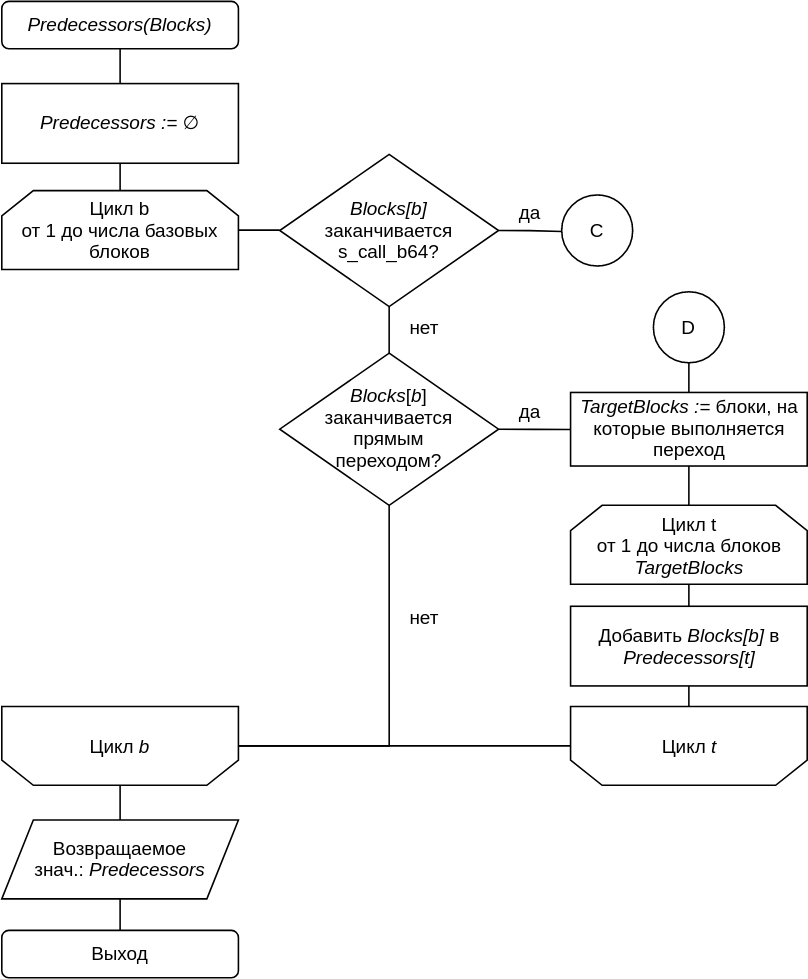
\includegraphics[width=0.75\textwidth]{diagrams/alg-cfg}
\caption{Блок-схема основного цикла опеределения предшественников}
\label{fig:diagram-cfg}
\end{figure}

Отдельно рассмотрим порядок обработки вызовов функций, обозначенный на схеме
соединителями $C$ и $D$. При условии, что пара регистров $RetGprs$, в которую
записывается адрес возврата, не изменяется при выполнении функции,
базовые блоки, из которых просходит возврат, можно определить статически.
Для этого необходимо отследить поток исполнения начиная с начала функции —
т.е. следовать по каждому прямому переходу до достижения возврата из функции
(\verb|s_setpc_b64|). Подробная схема алгоритма представлена на
на рисунке~\ref{fig:diagram-cfg-call}.

\begin{figure}[H]
\centering
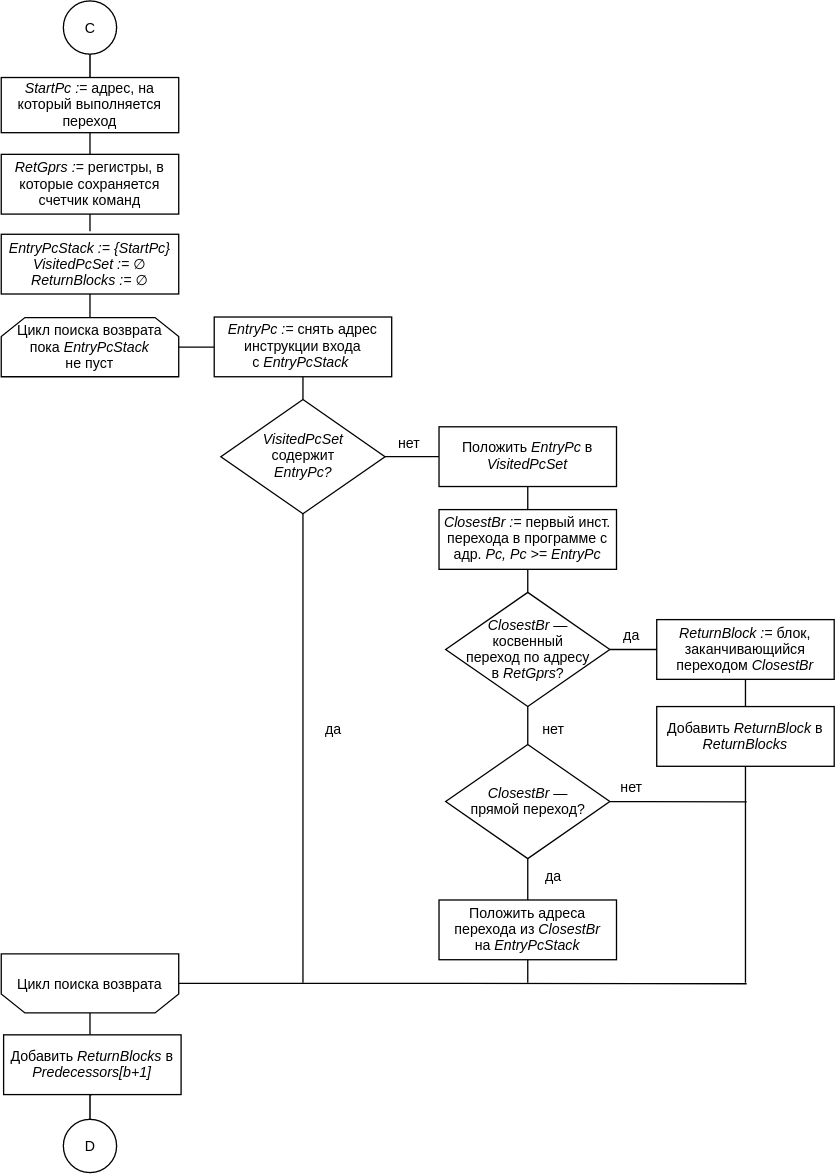
\includegraphics[width=\textwidth]{diagrams/alg-cfg-call}
\caption{Блок-схема опеределения предшественников при вызове функции}
\label{fig:diagram-cfg-call}
\end{figure}

Как видно из приведенной схемы, нахождение предшественников отдельной вершины
требует анализа всех остальных вершин графа, поэтому эта задача выполняется
на этапе восстановления потока управления.

Преемники вершины, в свою очередь, могут быть найдены во время обхода графа:
на каждой итерации достаточно вычислить адреса перехода из последней инструкции в текущем блоке.
Если инструкция является вызовом функции, то адрес возврата сохраняется, затем восстанавливается
при нахождении инструкции косвенного перехода (возврата из функции).

\subsubsection{Проверка инструкций ожидания запросов к памяти}

В ходе изучения подходов к статическому анализу было установлено, что верификация
вставки инструкций ожидания является проблемой анализа прямого потока данных.
При разработке алгоритма был выбран итеративный подход, аналогично реализации,
используемой в LLVM, рассмотренной в разделе~\ref{section:gcn-waitcnt-llvm}.

В отличие от реализации, используемой в LLVM, алгоритм сохраняет состояние всей очереди
незавершенных обращений. Для каждого из обращений хранится адрес инструкции, которая его
совершает, множество затрагиваемых регистров и тип запроса.

На рисунке~\ref{fig:diagram-waitcnt} приведена блок-схема основного цикла
алгоритма, который отвечает за обход управляющего графа. Для упрощения реализации
вместо RPO-обхода базовых блоков используется прямой обход в глубину.

На рабочий стек (\textit{WorkStack}) помещается базовый блок вместе с состоянием
очереди запросов к памяти на момент входа в него. На основании этой информации
процедурой \textit{AnalyzeInstructions} находится очередь запросов на момент
выхода из блока, которая становится входным состоянием для его преемников.

Помимо этого, каждый блок \textit{BB} ассоциируется с множеством выходных состояний,
для которых был совершен обход преемников (\textit{Visited[BB]}). Если текущее выходное
состояние уже было <<посещено>>, то обход преемников не выполняется.

\begin{figure}[H]
\centering
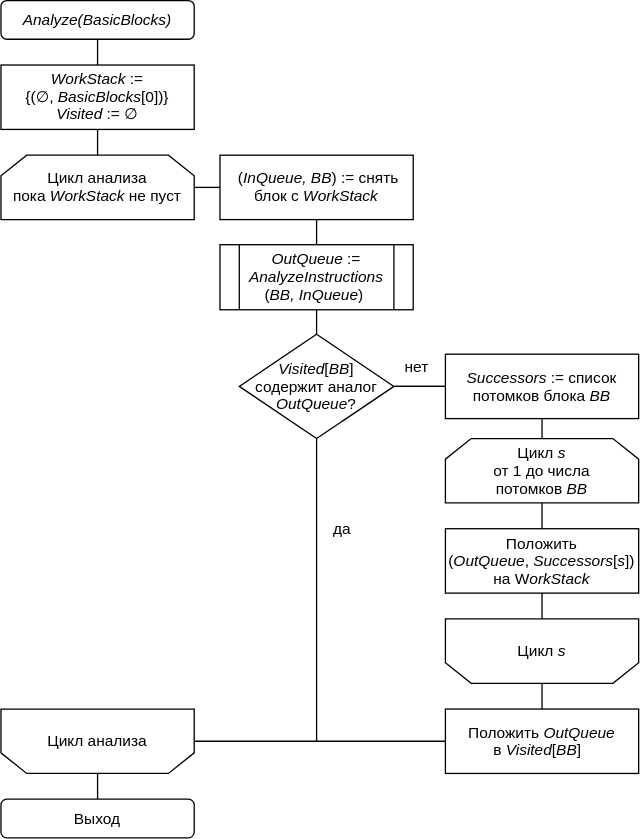
\includegraphics[width=0.8\textwidth]{diagrams/alg-waitcnt}
\caption{Блок-схема основного цикла проверки инструкций ожидания}
\label{fig:diagram-waitcnt}
\end{figure}

Рассмотрим подробнее работу процедуры \textit{AnalyzeInstructions}, блок-схема которой приведена
на рисунке~\ref{fig:diagram-waitcnt-analyze}. Она отвечает не только за нахождение нового состояния
очереди запросов к памяти, но и запись сообщений о найденных нарушениях — использовании результатов
обращений к памяти без соответвующего ожидания.

\begin{figure}[H]
\centering
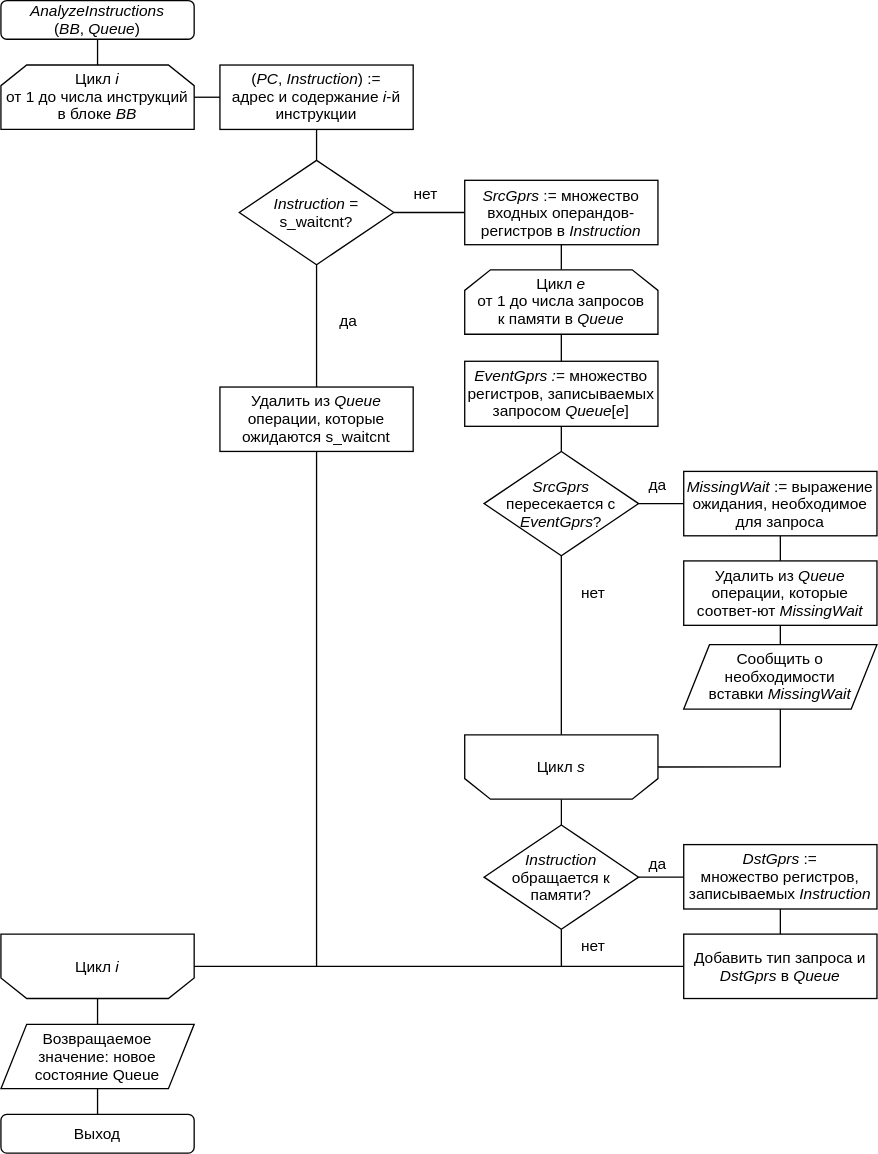
\includegraphics[width=\textwidth]{diagrams/alg-waitcnt-analyze}
\caption{Блок-схема анализа инструкций ожидания в отдельном блоке}
\label{fig:diagram-waitcnt-analyze}
\end{figure}\ %

Основной анализа выступает цикл, который проходит по всем инструкциям в блоке. Действие, совершаемое
на каждой итерации, зависит от типа рассматриваемой инструкции:

\begin{ul}
\item Инструкции ожидания счетчиков \texttt{s\_waitcnt}: из очереди удаляются
  запросы согласно выражению ожидания (см. раздел~\ref{section:gcn-waitcnt}).
\item Инструкции, содержащие регистровые операнды: для каждого из незавершенных запросов
  в очереди проверяется, есть ли среди регистровых операндов в инструкции те,
  которые записываются данным запросом. При обнаружении обращения к результату незавершенного
  запроса для него вычисляется выражение ожидания, которое сохраняется для
  дальнейшего вывода пользователю и применяется к очереди запросов. Таким образом,
  незавершенный запрос исключается из очереди, что предотвращает ее бесконечный
  рост и гарантирует конечность алгоритма.
\item Инструкции, выполняющие обращение к памяти: в очередь помещается информация о
  типе обращения, множестве записываемых регистров, адресе текущей инструкции.
\end{ul}

\subsubsection{Проверка слотов задержки между зависимыми инструкциями}

Алгоритм проверки слотов задержки повторяет подход, используемый в LLVM и рассмотренный
в разделе~\ref{section:gcn-wait-states-llvm}. Основным отличием является то, что алгоритм
сохраняет список инструкций, находящихся между зависимыми операциями. Данная информация
необходима для вывода сообщения об ошибке: программисту недостаточно знать адреса
зависимых операций, поскольку они могут находиться в разных частях программы, связанных
переходами.

В целях иллюстрации принципа работы алгоритма примем, что проверяется наличие
только одной конфликтной ситуации. Схема основного цикла представлена
на рисунке~\ref{fig:diagram-wait-states}.

\begin{figure}[H]
\centering
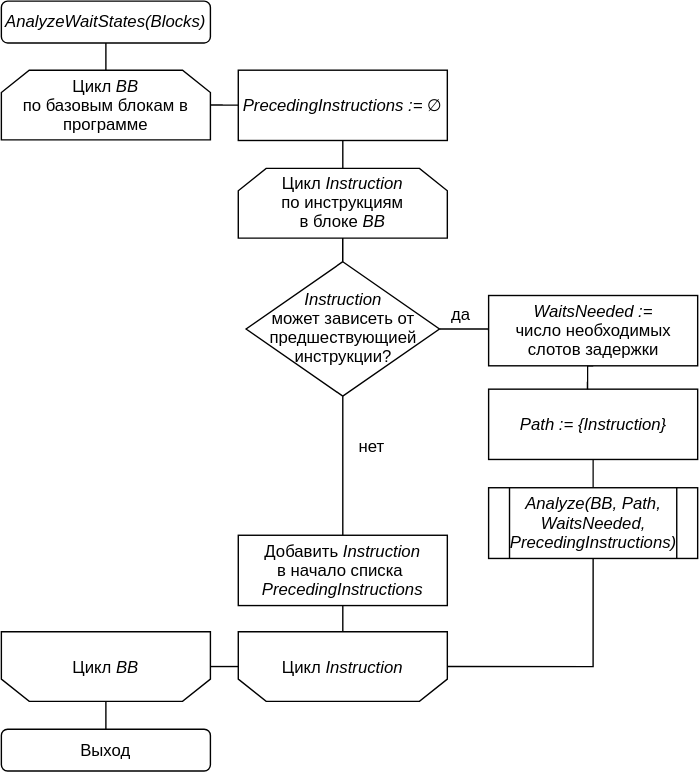
\includegraphics[width=0.8\textwidth]{diagrams/alg-wait-states}
\caption{Блок-схема основного цикла проверки слотов ожидания}
\label{fig:diagram-wait-states}
\end{figure}

Выполняется обход каждого базового блока в программе (порядок не важен),
при котором каждая инструкция проверяется на возможность конфликта
с предыдующими операциями. Если такая возможность существует,
то вызывается процедура анализа $\var{Analyze}$, которой передаются:
\begin{ul}
\item базовый блок (для определения предшественников при необходимости их обхода);
\item <<путь>> между зависимыми операциями, изначально содержащий проверяемую инструкцию;
\item число слотов задержки, которые необходимы при наличии конфликта;
\item список инструкций, предшествующих проверяемой, в порядке
от непосредственно предшествующей до первой в базовом блоке.
\end{ul}

Перейдем к процедуре анализа, схема которой изображена
на рисунке~\ref{fig:diagram-wait-states-analyze}.

\begin{figure}[H]
\centering
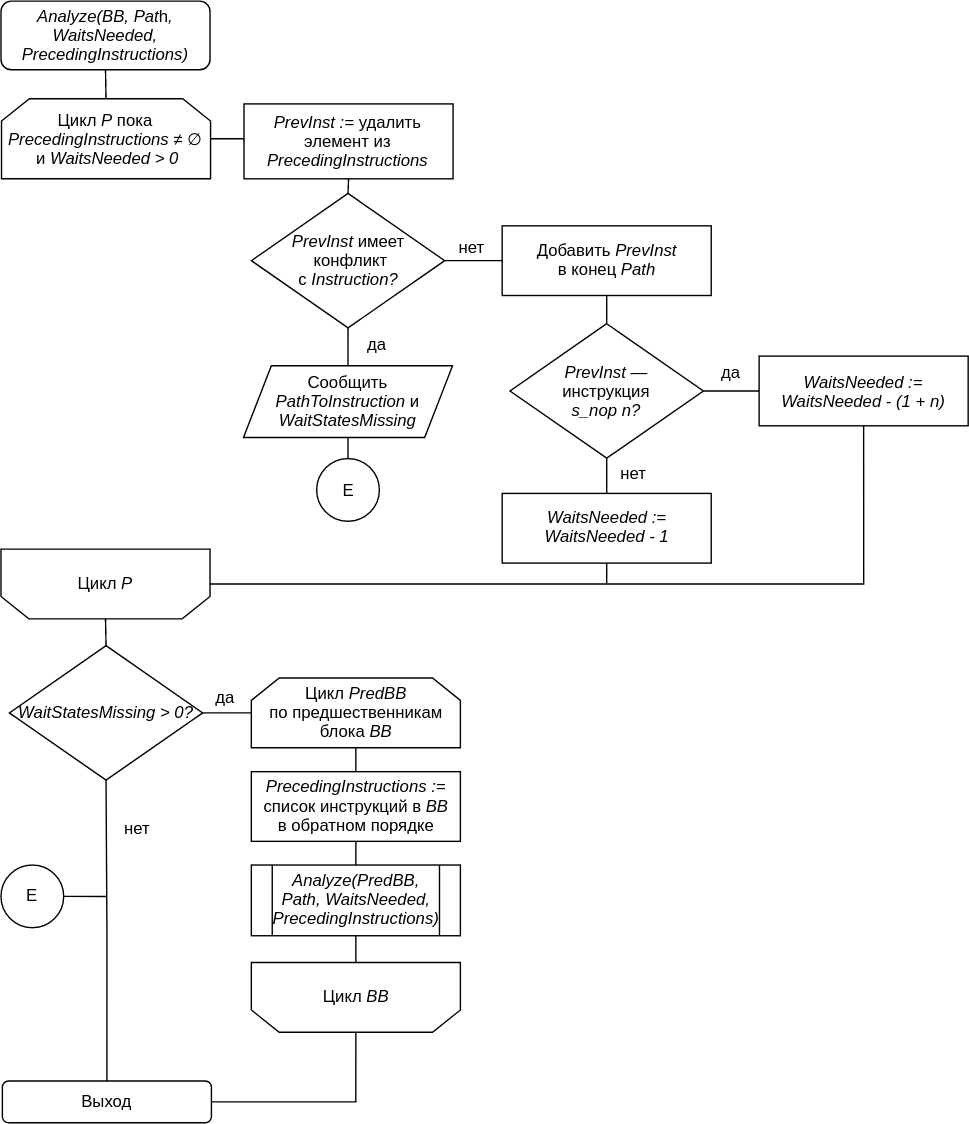
\includegraphics[width=\textwidth]{diagrams/alg-wait-states-analyze}
\caption{Блок-схема процедуры анализа отдельной инструкции}
\label{fig:diagram-wait-states-analyze}
\end{figure}

Сначала исследуются инструкции, предшествующие рассматриваемой в базовом блоке. 
При нахождении конфликта выводится сообщение об ошибке, процедура завершается.
Иначе независимая операция вычитается из числа необходимых слотов задержки
и записывается в путь между зависимыми операциями.

Если достигнуто начало базового блока, а число необходимых слотов задержки превышает 0,
то конфликт может быть найден в каком-либо из предшественников базового блока.
Для проверки каждого из них процедура анализа вызывается рекурсивно.

\newpage
\section{Создание программной реализации средства статического анализа}

\subsection{Проектирование архитектуры системы}
\label{section:system-design}

При проектировании архитектуры и выборе платформы для программной реализации
учитывались следующие особенности описанного подхода к статическому анализу:
\begin{ul}
\item Результат анализа однозначно определяется входным значением —
исполняемым файлом. Необходимость интерактивного ввода во время работы отсутствует.
\item Процесс анализа можно представить конвейером данных, состоящим из
последовательных этапов \textit{чтения исполняемого файла}, \textit{дизассемблирования},
\textit{восстановления управляющего графа}, \textit{непосредственно анализа}.
Выходные данные предыдущего этапа являются входными данными последующего этапа.
\end{ul}

Было принято решение использовать функциональный язык программирования Haskell,
позволяющий кратко и точно описать последовательность этапов анализа
путем составления и компоновки детерминированных (ссылочно прозрачных) функций.
Полученный код легко тестировать — достаточно составить пары входных и выходных
значений для каждого модуля. Компиляция программы в машинный код сокращает время
исполнения в десятки раз по сравнению с интерпретируемыми динамически типизированными
языками программирования\cite{rwhaskell}, такими как Python.
Это отражается на применимости системы в реальных задачах разработки —
чем больше времени занимает автоматический анализ шейдеров, тем реже он будет выполняться
программистом.

На рисунке~\ref{fig:diagram-arch} представлена диаграмма потока данных,
которая отражает основные компоненты системы, входные и выходные значения,
а также промежуточные артефакты.
%Пунктирной линией на схеме выделены 

\begin{figure}[H]
\centering
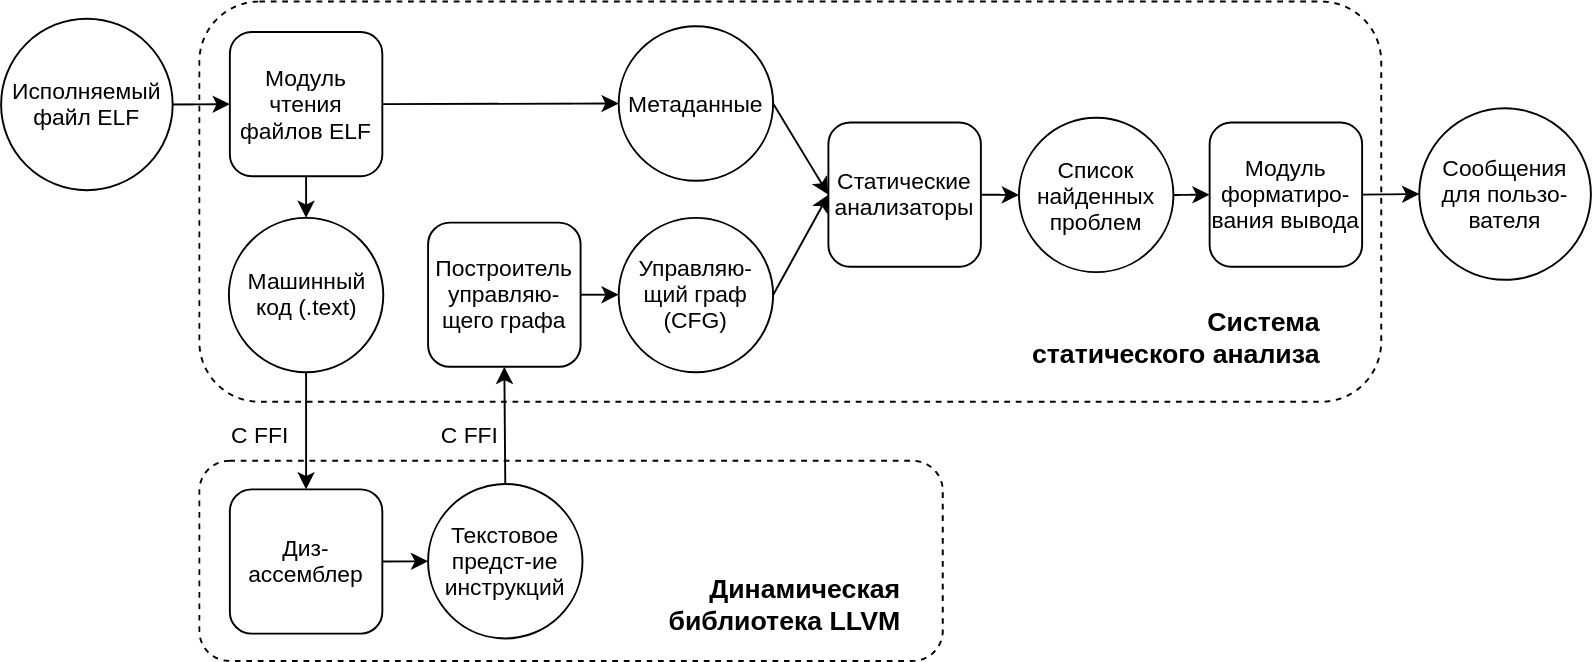
\includegraphics[width=1.01\textwidth]{diagrams/arch}
\caption{Диаграмма потока данных в разрабатываемой системе}
\label{fig:diagram-arch}
\end{figure}

Первым этапом реализации является определение междумодульных интерфейсов —
того, как в системе представляются промежуточные артефакты:

\begin{ol}
\item \textbf{Машинный код} считывается в массив байт (тип \verb|ByteString| в Haskell).
\item \textbf{Метаданные} шейдера — 256-байтный дескриптор в случае \textit{Code Object V2},
64-байтный дескриптор в случае \textit{Code Object V3} — также считываются в массив байтов. % N байт, массив байтов
В алгоритмах анализа, представленных в работе, метаданные не используются, однако они
могут понадобиться при разработке новых методов (см. раздел \ref{section:future-work}).
\item \textbf{Текстовое представление инструкции} является составным типом, включающим
в себя код операции и операнды. Очевидным решением для хранения кода операции
является строка — \verb|"s_cbranch_scc0"|, \verb|"v_cmp_eq_u32"| и т.д. Однако
стоит обратить внимание на то, что код операции состоит из нескольких частей:
\begin{ul}
\item \textit{класса операции}: \verb|s| — скалярные операции, \verb|v| — векторные операции и т.д.;
\item \textit{действия}: \verb|cbranch| — условный переход, \verb|cmp| — сравнение значений и т.д.;
\item \textit{дополнительных модификаторов}: \verb|scc0| — проверка флага \verb|SCC| на ноль,
\verb|eq| — проверка равенства значений и т.д.;
\item \textit{типа данных}: \verb|u32| — 32-разрядные беззнаковые целые числа, \verb|f32| —
числа с плавающей точкой одинарной точности (IEEE 754) и т.д.
\end{ul}
Представление кода операции в виде списка частей (например, \verb|["s", "cbranch", "scc0"]|)
облегчает поиск инструкций при анализе, поскольку проверка на равенство строк в конструкциях
сопоставления с шаблонами требует меньше кода, чем проверка на вхождение подстроки.

Операнды инструкций также делятся на классы — регистры, константные целые значения, константные
числа с плавающей запятой, выражения ожидания и т.д. Для эффективной работы с операндами
необходимо перевести их в вариантный тип:
\begin{verbatim}
data Operand = Osgpr [Int] | Ovgpr [Int]
             | Ovmcnt Int | Oexpcnt Int | Olgkmcnt Int
             | Oconst Int | Oconstf Float | Oother String
\end{verbatim}
\textit{При разработке новых методов анализа могут добавляться новые варианты. В текущей реализации
все неиспользуемые значения хранятся как вариант \texttt{Oother}.}

Удобство использования разработанного представления инструкций можно увидеть
на примере фрагмента кода, который обрабатывает переходы при восстановлении управляющего графа:
\begin{verbatim}
case instruction of
  Instruction ["s", "branch"] [Oconst off] ->
    -- Обработка безусловного перехода со смещением off
  Instruction ("s" : "cbranch" : _) [Oconst off] ->
    -- Обработка условного перехода со смещением off
  Instruction ("s" : "call" : _) [Osgpr [s1, s2], Oconst off] ->
    -- Обработка безусловного перехода со смещением off,
    -- при котором счетчик команд сохраняется
    -- в пару регистров с номерами (s1, s2)
\end{verbatim}

\item \textbf{Управляющий граф} представляет собой индексированный список базовых блоков,
  что позволяет хранить информацию о предшественниках и преемниках в виде пар индексов.

\item \textbf{Список найденных проблем} содержит элементы составного типа — каждому анализатору
соответствует свой вариант сообщения о проблеме.

При обнаружении пропущенной инструкции ожидания запроса к памяти сохраняется следующая информация:
\begin{ul}
\item регистры, которые используются незавершенным запросом;
\item адрес инструкции, которая читает результат незавершенного запроса;
\item состояние очереди обращений к памяти на момент чтения результата (влияет на выражение ожидания);
\item требуемое выражение ожидания;
\item краткое пояснение ошибки.
\end{ul}

При обнаружении пропущенных слотов задержки сохраняются:
\begin{ul}
\item адреса инструкций, между которыми необходимы дополнительные слоты задержки;
\item <<путь>> между зависимыми инструкциями, т.е. адреса команд, которые исполняются после исходной до зависимой:
это необходимо для лучшего понимания проблемы при наличии ветвления между зависимыми инструкциями;
\item инструкция, которую необходимо вставить для корректной работы программы:
как правило, это \verb|s_nop <wait states>|, где \verb|<wait states>| — число слотов задержки;
\item краткое пояснение ошибки.
\end{ul}

Общим элементом является адрес инструкции (\verb|PC|), нарушающей правило.
Поскольку он может использоваться для сортировки сообщений об ошибке, имеет смысл
хранить сообщения как пару из адреса и детального описания. Таким образом,
получим следующий тип сообщений об ошибках:
\begin{verbatim}
data Error = Error PC Violation

data Violation
  = CounterWaitRequired
      { ctrreqWaitcntClause :: Operand,
        ctrreqSucceedingEvents :: [(PC, String)],
        ctrreqPrecedingEvents :: [(PC, String)],
        ctrreqExplanation :: String
      }
  | WaitStatesRequired
      { wsreqMissingWaitStates :: Int,
        wsreqBacktrace :: [PC],
        wsreqExplanation :: String
      }
\end{verbatim}

\end{ol}

\todo{...}

\subsection{Интеграция модуля дизассемблера LLVM}
\label{section:impl-disasm}

\topic{Интерфейс прикладного программирования LLVM} Доступ к различным модулям LLVM
осуществляется через библиотеку LLVM-C. Использование дизассемблера осуществляется
в следущем порядке:
\begin{ol}
\item Инициализируется внутреннее состояние LLVM путем последовательного
вызова функций:
  \begin{ol}
  \item \verb|LLVMInitialize{TargetName}TargetInfo()|
  \item \verb|LLVMInitialize{TargetName}TargetMC()|
  \item \verb|LLVMInitialize{TargetName}Disassembler()|
  \end{ol}
Вместо \verb|{TargetName}| подставляется название бэкэнда, дизассемблер которого
используется — в нашем случае \verb|AMDGPU|.

\item Создается контекст дизассемблера для конкретного семейства процессоров
путем вызова функции \verb|LLVMCreateDisasmCPU| со следующими аргументами:
  \begin{ol}
  \item \verb|const char* Triple|: строка, идентифицирующая архитектуру и платформу.
Исполняемым файлам для ГП AMD на платформе ROCm соответсвует обозначение \verb|amdgcn--amdhsa|.
  \item \verb|const char* CPU|: строка, идентифицирующая семейство процессоров.
Ускорителю вычислений \textit{AMD Instinct MI100} соответствует обозначение \verb|gfx908|.
  \item \verb|void* DisInfo|: опциональный параметр для использования информации из таблицы
символов при дизассемблировании. В нашем случае не используется и выставляется в \verb|NULL|.
  \item \verb|int TagType|: опциональный параметр, см. выше. Выставляется в \verb|0|.
  \item \verb|LLVMOpInfoCallback GetOpInfo|: опциональный параметр, см. выше. Выставляется в \verb|NULL|.
  \item \verb|LLVMSymbolLookupCallback SymbolLookUp|: опциональный параметр, см. выше. Выставляется в \verb|NULL|. 
  \end{ol}

\item Производится считывание инструкций путем вызова функции
\verb|LLVMDisasmInstruction| со следующими аргументами:
  \begin{ol}
  \item \verb|LLVMDisasmContextRef DC|: непрозрачный указатель на контекст дизассемблера,
полученный на предыдущем этапе.
  \item \verb|uint8_t* Bytes|: указатель на начало области памяти с машинным кодом шейдера.
  \item \verb|uint64_t BytesSize|: размер области с машинным кодом шейдера.
  \item \verb|uint64_t PC|: смещение считываемой инструкции относительно начала шейдера.
  \item \verb|char* OutString|: указатель на область памяти, в которую будет записано
текстовое представление инструкции.
  \item \verb|size_t OutStringSize|: размер области памяти для записи текстового представления инструкции.
  \end{ol}
Функция возвращает число байт в считанной инструкции, то есть для дизассемблирования всего шейдера необходим цикл,
в котором к переменной $\var{PC}=0$ прибавляется возвращаемое значение \verb|LLVMDisasmInstruction| до
достижения конца программы.
Стоит учитывать, что возвращаемое значение равно нулю, если инструкция не распознана. Отсутсвие проверки
может привести к бесконечному циклу.

\item По завершении дизассемблирования ресурсы LLVM освобождаются из памяти вызовом
функции \verb|LLVMDisasmDispose|, которая принимает в качестве аргумента
непрозрачный указатель на контекст дизассемблера.
\end{ol}

\topic{Взаимодействие с подключаемыми библиотеками в Haskell} Привязка к функциям,
вызываемым из внешних библиотек, реализуется специальным языковым расширением
\cite[Глава~17]{rwhaskell}, которое включается директивой
\verb|{-# LANGUAGE ForeignFunctionInterface #-}|.

Рассмотрим декларацию одной из функций ининциализации внутреннего состояния LLVM:
\begin{verbatim}
foreign import ccall
  "llvm-c/Target.h LLVMInitializeAMDGPUTargetInfo"
  llvmInitializeAMDGPUTargetInfo :: IO ()
\end{verbatim}

В конструкции \verb|foreign import| указывается соглашение о вызовах, которое будет
использовано для обращения к внешней функции — \verb|ccall| соответствует соглашению языка С.
Затем задается заголовочный файл, содержащий сигнатуру внешней функции, и ее название.
Наконец объявляется имя функции на языке Haskell, типы ее аргументов и результата.
В приведенном примере тип функции указан как \verb|IO ()|, приблизительно соответствующий
\verb|void| в C. Это означает, что функция не принимает аргументов и не возвращает результат,
но имеет побочные эффекты — изменяет глобальное состояние.
Монада \verb|IO| гаранирует, что оптимизации компилятора не затронут порядок вызова функции
относительно других действий с побочными эффектами\cite[Глава~7]{rwhaskell}.\\

Перейдем к инициализации контекста дизассемблера:
\begin{verbatim}
foreign import ccall
  "llvm-c/Disassembler.h LLVMCreateDisasmCPU"
  llvmCreateDisasmCPU :: CString -> CString ->
    Ptr () -> CInt -> Ptr () -> Ptr () -> IO (Ptr ())
\end{verbatim}

Поскольку в Haskell используется автоматическое управление памятью,
ручное отслеживание времени жизни внешних ресурсов
может привести к утечкам памяти или ошибкам \textit{use-after-free}.
Сборщик мусора может автоматически освободить внешний ресурс, если он
обернут в тип \verb|ForeignPtr|, который также хранит указатель на функцию
освобождения. Для получения указателя на функцию перед ее именем ставится символ \verb|&|:
\begin{verbatim}
foreign import ccall
  "llvm-c/Disassembler.h &LLVMDisasmDispose"
  llvmDisasmDispose :: FunPtr (Ptr () -> IO ())
\end{verbatim}

Объявим функцию создания контекста дизассемблера, которая скрывает детали
реализации (преобразование типов для передачи в C, управление памятью, инициализацию
глобального состояния):
\begin{verbatim}
type LLVMDisasmContextRef = ForeignPtr ()

createCtx :: String -> String -> IO LLVMDisasmContextRef
createCtx llvmTriple llvmCpu = do
  llvmInitializeAMDGPUTargetInfo
  llvmInitializeAMDGPUTargetMC
  llvmInitializeAMDGPUDisassembler
  withCString llvmTriple $ \tripleStr ->
    withCString llvmCpu $ \cpuStr -> do
      ctxRefRaw <- llvmCreateDisasmCPU tripleStr cpuStr
        nullPtr 0 nullPtr nullPtr
      newForeignPtr llvmDisasmDispose ctxRefRaw
\end{verbatim}

Если примитивные значения (\verb|Int|) могут быть автоматически переведены
в соответствующие типы C, то со строками такое преобразование невозможно.
Тип \verb|char*| в C является указателем на область памяти, которая содержит символы
строки и заканчивается нулевым байтом. Стандартный тип \verb|String| в Haskell,
в свою очередь, реализован как связный список символов. Для передачи строк
используется функция \verb|withCString|, которая выделяет новую область в памяти,
копирует в нее элементы списка и добавляет нулевой байт. Указатель передается
в лямбда-выражение, которое совершает \verb|IO| действие со строкой. По завершении
действия временная копия строки удаляется из памяти.

\todo{LLVMDisasmInstruction}

\subsection{Реализация и тестирование алгоритмов анализа}

Алгоритмы восстановления управляющего графа, анализа обращений к памяти и анализа
вставки слотов задержки подробно описаны в главе <<\nameref{section:algorithms}>>.
Их трансляция в исходный код является несложным процессом и не представляет
теоретического интереса.

Корректность реализации проверяется при помощи автоматических тестов,
написанных с применением фреймворка \verb|Hspec|. Тестовые сценарии состоят
из небольшого ассемблерного листинга и ожидаемого результата
анализа. Запуск тестовых сценариев осуществляется в следующем порядке:
\begin{ol}
\item Создается временная директория \verb|$(TmpDir)|, в которую сохраняется файл
с листингом \verb|test.s|.
\item Запускается компилятор \textit{Clang}, который создает исполняемый файл
\verb|test.co|, при помощи следующей команды:
\begin{verbatim}
docker run --user=root -v $(TempDir):/out:z -w=/out rocm/rocm-terminal:4.1.1 /opt/rocm/llvm/bin/clang -x assembler -target amdgcn--amdhsa -mcpu=gfx908 -mcode-object-version=3 -o test.co test.s
\end{verbatim}

Поскольку платформа ROCm имеет жесткие требования к используемой операционной системе,
компилятор запускается в контейнере с официально поддерживаемым образом платформы (\verb|rocm/rocm-terminal:4.1.1|).
Данный подход облегчает настройку тестовой среды: исключаются ошибки из-за несовместимости версий \textit{Clang},
возможно использование любого дистрибутива \textit{Linux}, в котором установлен \textit{Docker Engine}.

\item Полученный исполняемый файл \verb|$(TmpDir)/test.co| подается на вход тестируемого модуля.
\item Вывод модуля сверяется с ожидаемым результатом.
\end{ol}

Рассмотрим пример тестового сценария для модуля проверки запросов к памяти.
Вспомогательная функция \verb|loadGfx908Kernel| создает исполняемый файл,
содержащий заданный листинг, затем дизассемблирует его и
восстанавливает управляющий граф. Функция \verb|checkWaitcnts| реализует
алгоритм анализа: она принимает на вход метаданные, \verb|kernel|, и управляющий
граф, \verb|cfg|, и возвращает список найденных ошибок. Вспомогательная функция
\verb|shouldBe| проверяет соответствие результата ожидаемому значению.

Каков ожидаемый результат? Во входном шейдере присутствует два
обращения к памяти: запись регистров \verb|v[0:3]| и \verb|v[4:7]|.
Команда по адресу 16 перезаписывает регистр \verb|v0| результатом сложения
\verb|v2| и константы \verb|1.0|. Поскольку \verb|v2| был считан из памяти,
перед его использованием должна быть команда ожидания завершения операции.
Модуль проверки должен сообщить об ее отсутствии.

\begin{verbatim}
spec :: Spec
spec = describe "dependency resolution using s_waitcnt" $ do
  it "checks vector memory reads with buffer instructions" $ do
    (cfg, kernel) <-
      loadGfx908Kernel "waitcnt_buffer_load" $
        [i|
          buffer_load_dwordx4 v[0:3], off, s[0:3], 0            // PC 0
          buffer_load_dwordx4 v[4:7], off, s[0:3], 0 offset:16  // PC 8
          v_add_f32 v0, v2, 1.0                                 // PC 16
        |]
    checkWaitcnts kernel cfg `shouldBe` [
      Error 16 CounterWaitRequired
        { ctrreqWaitcntClause = Ovmcnt 1
        , ctrreqSucceedingEvents =
            [(8, "(0) vmem access: v4, v5, v6, v7")]
        , ctrreqPrecedingEvents =
            [(0, "(1) vmem access: v0, v1, v2, v3")]
        , ctrreqExplanation =
            "Source register v2 is read from memory. " ++
            "The operation is complete when the counter reaches 1 " ++
            "because there is one operation enqueued after it."
        }
   ]
\end{verbatim}

Тип, используемый для представления сообщения о нарушении, описан в разделе
\ref{section:system-design}.

\todo{...}

Оценка тестового покрытия была проведена при помощи инструмента \textit{Haskell Program Coverage}.
Результаты оценки представлены в таблице \ref{table:test-coverage}.

\begin{table}[H]
\caption{Оценка тестового покрытия модулей системы}
\label{table:test-coverage}
\begin{tabular}{|l|l|l|}
\hline
\thead{Название модуля \\ (предназначение)} & \thead{Кол-во тестовых \\ сценариев} & \thead{Степень \\ покрытия кода} \\\hline
\makecell[l]{\texttt{Disassembler.ElfReader}\\[2mm] (Чтение исполняемых файлов ELF)} & 2 & 100\% \\\hline
\makecell[l]{\texttt{Disassembler.InstructionParser}\\[2mm] (Трансляция операндов инструкций\\из строк в составной тип)} & 6 & 95\% \\\hline
\makecell[l]{\texttt{ControlFlow}\\[2mm] (Восстановление управляющего графа)} & 3 & 96\% \\\hline
  \makecell[l]{\texttt{Analysis.Waitcnt}\\[2mm] (Проверка инструкций ожидания\\запросов к памяти)} & 5 & 92\% \\\hline
\makecell[l]{\texttt{Analysis.WaitStateHazard}\\[2mm] (Проверка слотов задержки\\между зависимыми инструкциями)} & 4 & 94\% \\\hline
\end{tabular}
\end{table}

\subsection{Проверка работы системы, анализ результатов}

Применимость системы в реальных задачах разработки оценивается с использованием
существующих ассемблерных шейдеров, реализующих примитивы для глубинного обучения
в открытом проекте MIOpen\cite{miopen}.

Проверка алгоритма вставки инструкций ожидания выполняется следующим образом:
существующие в шейдере инструкции \verb|s_waitcnt| поочередно заменяются на
пропуски (\verb|s_nop|), затем вывод системы вручную сопоставляется с ожидаемыми
сообщениями о нарушениях.

В качестве примера взят шейдер, реализующий операцию свертки — \verb|Conv_Winograd|.
Сборка исполняемого файла производится последовательностью команд:

\begin{verbatim}
git clone --depth 1 --branch rocm-4.1.0 \
  https://github.com/ROCmSoftwarePlatform/MIOpen
cd MIOpen/src/kernels/
/opt/rocm/llvm/bin/clang -x assembler \
  -target amdgcn--amdhsa -mcpu=gfx908:xnack- \
  -mcode-object-version=3 -o winograd.co \
  Conv_Winograd_v21_1_2_fp32_stride1.s
\end{verbatim}

Для запуска тестов в консольном приложении анализа предусмотрена опция
\verb|--nop=<addr>|, которая при дизассемблировании шейдера автоматически
заменяет инструкцию по адресу \verb|<addr>| на \verb|s_nop|.

Будем считать, что система корректно распознает нарушение при вставке инструкций
ожидания, если соблюдены следующие условия:
\begin{ul}
\item сообщение об ошибке ссылается на адрес первой инструкции, использующей результат
обращения к памяти без ожидания;
\item сообщение об ошибке ссылается на адрес инструкции, совершающей требуемое обращение к памяти;
\item сообщение об ошибке указывает на регистр, участвующий в зависимых операциях.
\item сообщение об ошибке указывает на значение соответствующего счетчика операций,
после ожидания которого регистр гарантированно содержит результат операции.
\end{ul}

В таблице \ref{table:test-waitcnt-winograd} представлены адреса инструкций ожидания
в программе, их предназначение и поведение системы при замене инструкции на \verb|s_nop|.

Как видно из результатов, система не распознает пропуск инструкции ожидания как ошибку только
в одном случае: когда \verb|s_waitcnt| находится перед инструкцией \verb|s_barrier|. Действительно,
алгоритм анализа не рассматривает данный случай, поскольку он не описан в официальном руководстве
к архитектуре CDNA\cite{cdna-isa}.

Для остальных нарушений вывод системы полностью соответствует критериям корректности, описанным
выше. Стоит обратить внимание на то, что предлагаемое выражение ожидания не всегда совпадает
с тем, которое было изначально указано в шейдере. Подобное несоответствие объясняется тем,
что при наличии несколько идущих подряд команд, использующих результаты запросов к памяти,
программист как правило вставляет одно ожидание, наиболее строгое — т.е. покрывающее все
необходимые операции. Система же при вычислении необходимого ожидания опирается только
на одну инструкцию — первую, для которой обнаружено нарушение. \todo{переформулировать}

\begin{table}[H]
  \caption{Поведение системы при пропуске инструкций ожидания в шейдере \texttt{Conv\_Winograd}}
\label{table:test-waitcnt-winograd}
\begin{tabular}{|l|p{2.8cm}|p{6.5cm}|p{5cm}|}
\hline
\textbf{Адрес} & \textbf{Выражение ожидания} & \textbf{Предназначение} & \textbf{Поведение системы при замене на s\_nop} \\\hline
0x58 & \verb|0|
  & Ожидание перед барьером синхронизации \texttt{0x5C: s\_barrier}
  & Нарушение не обнаружено \\\hline
0x8C & \verb|lgkmcnt(0)|
  & Инструкция \verb|0x98| читает регистр \verb|s21| после команды \verb|0x74|: \verb|s_load_dwordx16|
  & Нарушение распознано, предложено выражение \verb|lgkmcnt(0)| \\\hline
0x16C & \verb|lgkmcnt(0)|
  & Инструкция \verb|0x170| читает регистр \verb|s35| после команды \verb|0xE0|: \verb|s_load_dwordx2|
  & Нарушение распознано, предложено выражение \verb|lgkmcnt(0)| \\\hline
0x1EC & \verb|lgkmcnt(0)|
  & Инструкция \verb|0x1F0| читает регистр \verb|s21| после команды \verb|0xB8|: \verb|s_load_dwordx2|
  & Нарушение распознано, предложено выражение \verb|lgkmcnt(0)| \\\hline
0xB0C & \verb|lkmcnt(5)|
  & Инструкция \verb|0xB20| читает регистр \verb|v38| после команды \verb|0x16C0|: \verb|ds_read_b128|
  & Нарушение распознано, предложено выражение \verb|lgkmcnt(11)| \\\hline
0xBFC & \verb|vmcnt(12)| \verb|lgkmcnt(5)|
  & Инструкция \verb|0xC20| читает регистр \verb|v34| после \verb|0xAAC|: \verb|ds_read_b128| (счетчик \textit{lgkmcnt});
  инструкция \verb|0xC98| читает регистр \verb|v70| после \verb|0x1160|: \verb|buffer_load_dword| (счетчик \textit{vmcnt})
  & Нарушения обнаружены отдельно для каждого счетчика, предложены выражения \verb|lgkmcnt(11)| и \verb|vmcnt(15)| \\\hline 
... & ... & Повторение инструкций \texttt{0xB0C} и \texttt{0xBFC} (развернутый цикл) & Идентично описанному выше \\\hline
0x3080 & \verb|vmcnt(0)|
  & Инструкция \verb|0x3084| читает регистр \verb|v104| после команды \verb|0x34FC|: \verb|buffer_load_dword|
  & Нарушение обнаружено, предложено выражение \verb|vmcnt(3)| \\\hline
0x33B4 & \verb|lgkmcnt(0)|
  & Инструкция \verb|0x33B8| читает регистр \verb|v86| после команды \verb|0x3394|: \verb|ds_read_b32|
  & Нарушение обнаружено, предложено выражение \verb|lgkmcnt(0)| \\\hline
\end{tabular}
\end{table}

\todo{Сравнить с SIInsertWaitcnts}

\subsection{Дальнейшие направления работы}
\label{section:future-work}

Описанный алгоритм учета обращений к памяти является частным случаем анализа потока данных,
т.е. того, какие значения встречаются на различных этапах исполнения. В компиляторах
анализ потока данных используется для поиска оптимизаций, часть из которых применима и к
ассемблерным шейдерам.

Рассмотрим в качестве примера гипотетический анализ времени жизни регистров. Если алгоритм
статически доказывает, что времена жизни значений в двух регистрах не пересекаются, то
в программе может использоваться только один из них. Результатом оптимизации
является сокращение общего числа регистров, что приведет к увеличению утилизации аппаратных ресурсов:
на одном и том же CU будет запущено большее число инстанций шейдера\cite{gcn-performance}.

Помимо этого, интересен анализ возможных диапазонов значений, с помощью которого можно статически
обнаружить вероятное переполнение или выход за границы массива.

\todo{...}

\newpage
\section*{ЗАКЛЮЧЕНИЕ}
\phantomsection\addcontentsline{toc}{section}{ЗАКЛЮЧЕНИЕ}

В работе проведен обзор архитектурных особенностей графических процессоров,
требующих специальных вставок в коде шейдеров, и их обработки при компиляции
высокоуровневых языков. Исследованы теоретические основы статического анализа
кода. Обосновано применение статического анализа для облегчения ручного составления
ассемблерных шейдеров. Определены цель и задачи работы.

На основании произведенного исследования выдвинут подход к статическому анализу
исполняемых файлов шейдеров. Разработан алгоритм восстановления управляющего
графа шейдеров, учитывающий прямые и (статически разрешимые) косвенные переходы
в программе. Составлены алгоритмы верификации шейдеров, которые основываются на
существующих методах, используемых в компиляторах, но вносят в них значимые изменения.

При создании программной реализации алгоритмов спроектирована архитектура системы
для статической верификации шейдеров. Решены такие практические вопросы, как
дизассемблирование машинного кода для различных семейств графических процессоров,
модульное тестирование алгоритмов. Произведена апробация системы на существующем
ассемблерном шейдере, в ходе которой продемонстрировано, что система способна
не только обнаружить ошибки, но и предоставить программисту на ассемблере всю
необходимую информацию для решения проблемы. Рассмотрены возможные направления
дальнейшего развития проекта.

Таким образом, результатом работы является система статической верификации исполняемых
файлов для графических процессоров, которая позволяет обнаруживать ошибки в обработке
запросов к памяти и вставке слотов задержки при разработки ассемблерных шейдеров.
Исходный код и инструкция по использованию системы размещены в публичном доступе
на портале GitHub: \verb|...|

\newpage
\phantomsection
\addcontentsline{toc}{section}{СПИСОК ИСПОЛЬЗОВАННЫХ ИСТОЧНИКОВ}
\selectlanguage{russian}
\printbibliography[title={СПИСОК ИСПОЛЬЗОВАННЫХ ИСТОЧНИКОВ}]

\end{document}
